\documentclass[10pt, reqno]{amsart}
\usepackage[margin = 0.5 in]{geometry}
\usepackage{multicol}
\usepackage{float}
\usepackage{fancyhdr}
\usepackage{graphicx}
\usepackage{hyperref}
\usepackage{fancyvrb}
\usepackage{physics}

\setlength{\abovecaptionskip}{5pt plus 3pt minus 3pt}

\hypersetup{colorlinks=true,allcolors=blue}
\pagestyle{fancy} \fancyhead{} \fancyfoot[C]{\normalsize\thepage}
\renewcommand{\headrulewidth}{0pt}
\begin{document}
\title{ME 5311 \quad Assignment 4 \quad Jacob Ivanov}

\maketitle
\begin{multicols}{2}
    \section{Spectral Differentiation Matrix}
    \begin{equation}
        \hat{\delta}_n = \mathrm{DFT} \left[ \delta_i \right] = \sum_{i = 0}^{N - 1} \left[ \delta_i e^{-\underline{i} k_n x_i} \right]
    \end{equation}
    $k_n$ can be simplifed as $k_n = 2 \pi n / (2 \pi) = n$
    \begin{equation}
        \begin{aligned}
        \hat{\delta}_n &= \left( \delta_0 e^{-\underline{i} n x_0} \right) + \left( \delta_1 e^{-\underline{i} n x_1} \right) + \ldots + \left( \delta_{N-1} e^{-\underline{i} n x_{N-1}} \right) \\
        &= \left( \delta_0 e^{-\underline{i} n x_0} \right) = 1e^0 = 1
        \end{aligned}
    \end{equation}
    We can then construct the polynomial interpolations as the following:
    \begin{equation}
        p(x) = \frac{1}{2N} \sum_{n = - \frac{N}{2}}^{\frac{N}{2}-1} \left[ \hat{\delta}_n e^{\underline{i} n x} \right] + \frac{1}{2N} \sum_{n = - \frac{N}{2} + 1}^{\frac{N}{2}} \left[ \hat{\delta}_n e^{\underline{i} n x} \right]
    \end{equation}
    By using general formula for an exponential sum, we can simplify this to:
    \begin{equation}
        p(x) = \frac{1}{N} \left[ \frac{e^{\underline{i} x \left(-\frac{N}{2}\right)} - e^{\underline{i} x \left(+\frac{N}{2}\right)}}{2 \left(1 - e^{\underline{i} x} \right)} + \frac{e^{\underline{i} x \left(-\frac{N}{2} + 1\right)} - e^{\underline{i} x \left(+\frac{N}{2} + 1\right)}}{2 \left(1 - e^{\underline{i} x} \right)} \right]
    \end{equation}
    By using Euler's Identity, this can be changed to:
    \begin{equation}
        p(x) = \frac{1}{N} \frac{\sin \left( \frac{N x}{2} \right) \left( \sin(x) - \underline{i} \cos(x) \right) - \underline{i} \sin \left( \frac{N x}{2} \right)}{1 - \underline{i} \sin(x) - \cos(x)}
    \end{equation}
    \begin{equation}
        p(x) = \frac{1}{N} \sin \left( \frac{N x}{2} \right) \left[ \frac{\sin(x) - \underline{i} \cos(x) - \underline{i}}{1 - \underline{i} \sin(x) - \cos(x)} \right]
    \end{equation}
    \begin{equation}
        p(x) = \frac{1}{N}\sin \left( \frac{N x}{2} \right) \cot \left( \frac{x}{2} \right)
    \end{equation}
    From which, the continuous derivative can be found to be:
    \begin{equation}
        p'(x) = \frac{N \cot \left( \frac{x}{2} \right) \cos \left( \frac{Nx}{2} \right) - \csc^2 \left( \frac{x}{2} \right) \sin \left( \frac{Nx}{2} \right)}{2N}
    \end{equation}
    And the discrete derivative can be found as follows:
    \begin{equation}
        p'_{\mathrm{TS}}(x_i) = -\frac{1}{12} (N^2 + 2) x_i + \mathcal{O}(x_i^2) \to p'_{\mathrm{TS}}(0) = 0
    \end{equation}
    Though the continous function away from $x_i = 0$ can be visually shown to agree with the discrete version, I was not completely sure how to manipulate them to show that algebraicly.
    \begin{equation}
        \frac{N \cot \left( \frac{x}{2} \right) \cos \left( \frac{Nx}{2} \right) - \csc^2 \left( \frac{x}{2} \right) \sin \left( \frac{Nx}{2} \right)}{2N} = \frac{1}{2} (-1)^i \cot \left( \frac{\pi i}{N} \right)
    \end{equation}

    \begin{figure}[H]
        \centering
        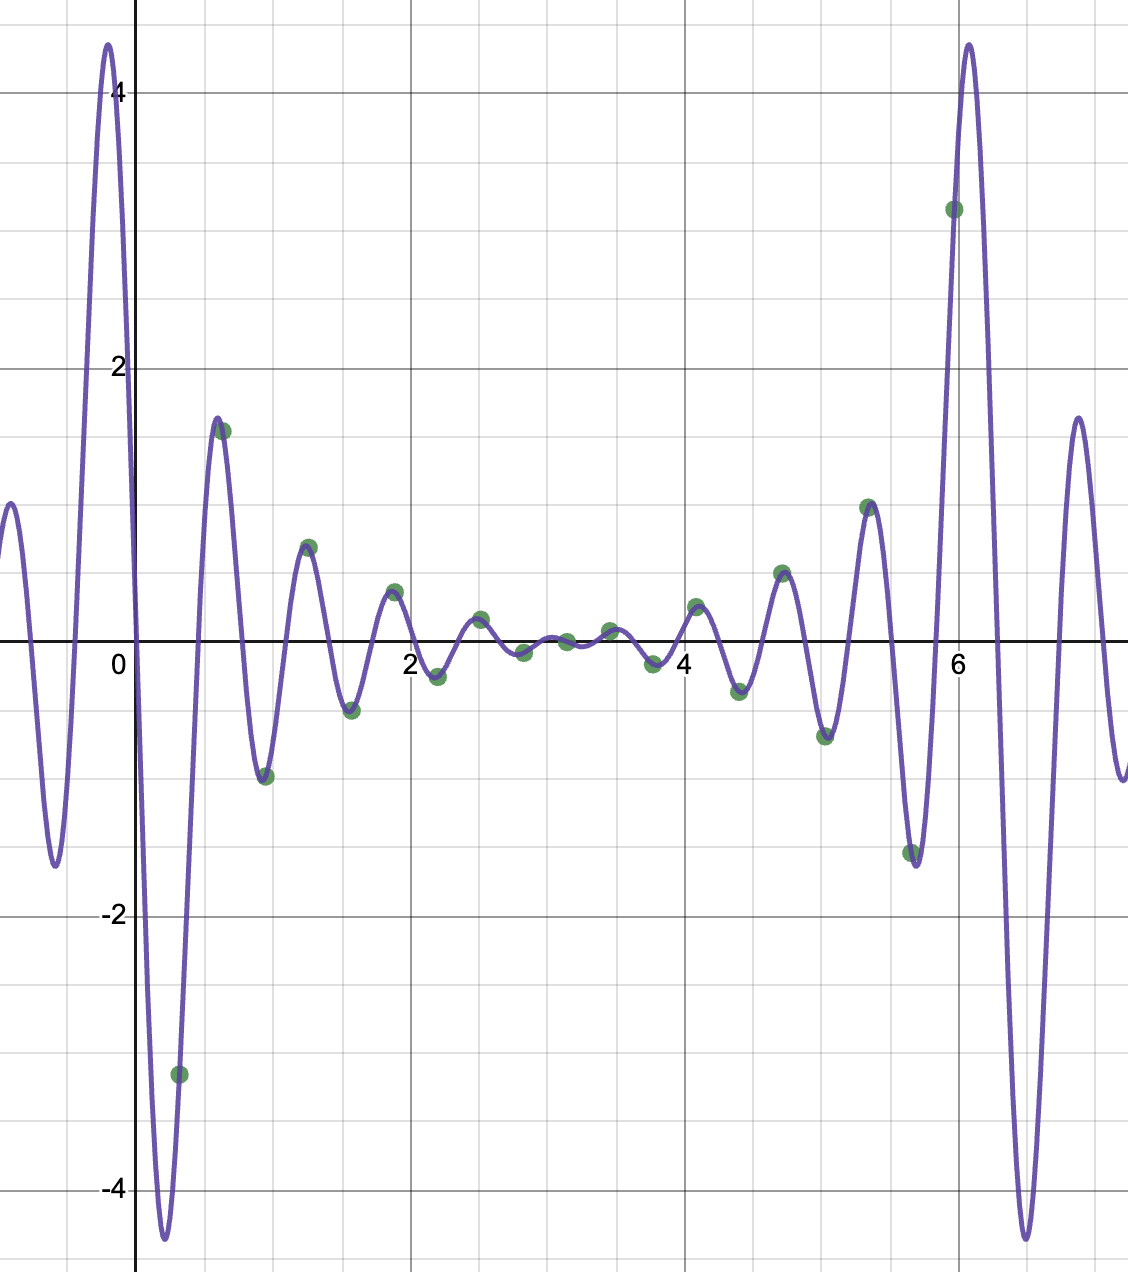
\includegraphics[width = 0.7\linewidth]{DFT Proof by Desmos.png}
    \end{figure}

    \begin{equation}
        p'(x_i) = \begin{cases}
            0, \quad i = 0 \\
            \frac{1}{2} (-1)^i \cot \left( \frac{i \Delta x}{2} \right), \quad i \neq 0 \end{cases}
    \end{equation}

    \section{Comparison of Derivative Approximations}

    \begin{figure}[H]
        \centering
        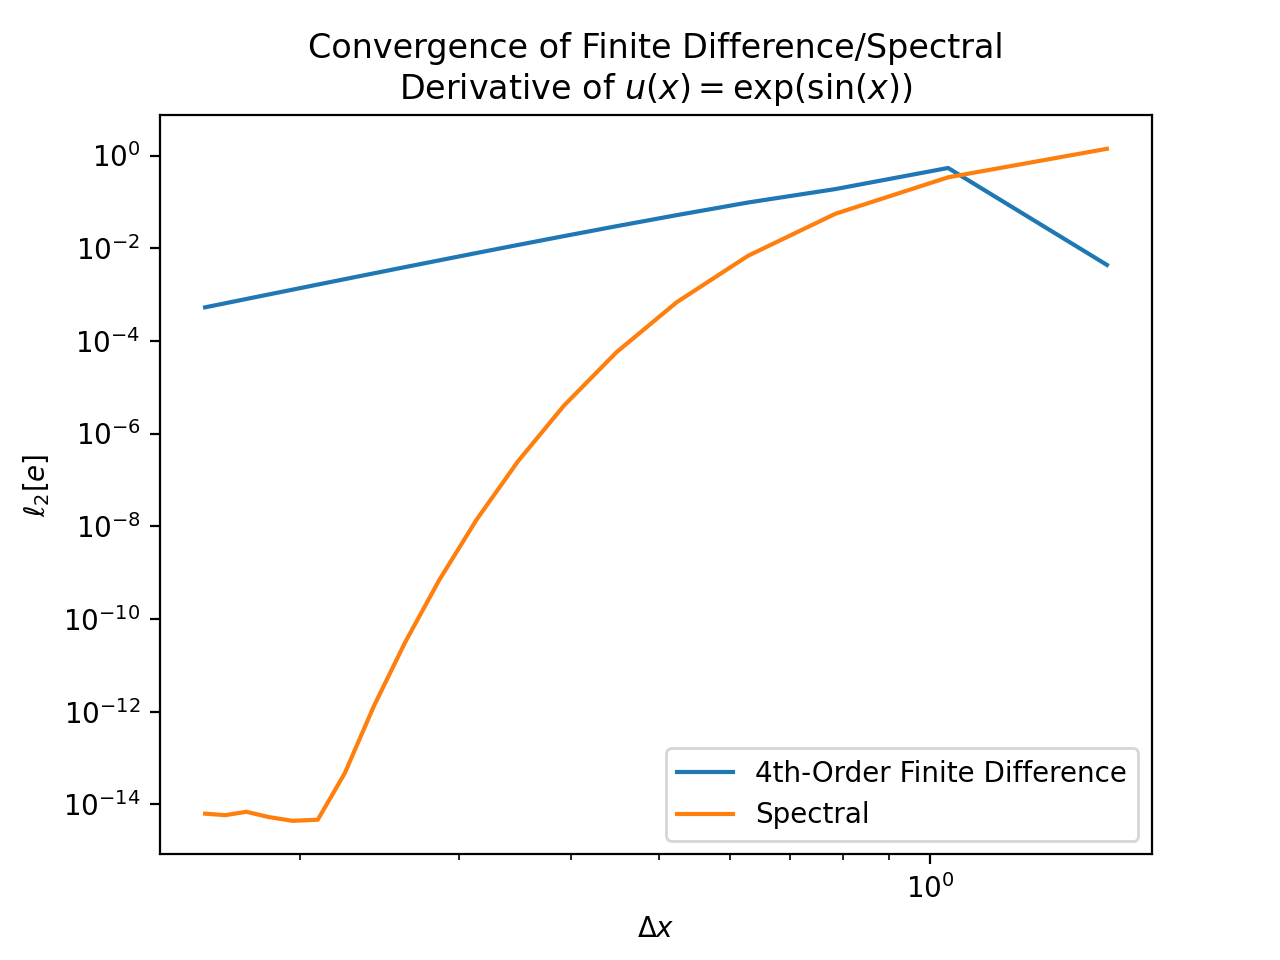
\includegraphics[width=1\linewidth]{Convergence of Derivatives.png}
    \end{figure}
    As can be seen from the figure above, the spectral derivative error rapidly converges to machine epsilon with a non-constant order, whereas the 4th Order Finite Difference has a constant order. It should be noted that the error in the FDM for larger timesteps is due to the fact that convergence is asymptotic. When $\Delta x$ is large, it can vary from the actual convergence rate.
\end{multicols}
\end{document}